%%%%%%%%%%%%%%%%%%%%%%%%%%%%%%%%%%%%%%%%%%%%%%%%%%%%%%%%%%%%%%%%%%%%%%%%%%%
%%%%%%%%%%%%%%%%%%%%%%%%%%%%%%%%%%%%%%%%%%%%%%%%%%%%%%%%%%%%%%%%%%%%%%%%%%%
%%
%% The basic tex file for the header of all the lectures. 
%%

\documentclass{beamer}
\usetheme[hideallsubsections]{Berkeley}

\usepackage{color}
\usepackage{amsfonts}

\definecolor{myblue}{rgb}{0.25, 0, 0.75}
\definecolor{mygold}{rgb}{1,0.8,0.2}
\definecolor{gray}{rgb}{0.5, 0.5, 0.5}
\definecolor{lucia}{rgb}{0.8,0.4,0.7} 

\newcommand{\myurl}[1]{\href{http://#1}{\textcolor{gray}{\texttt{#1}}}}
\newcommand{\myem}[1]{\structure{#1}}
\newcommand{\RPack}[1]{\textcolor{gray}{\textsf{#1}}}
\newcommand{\pl}[1]{\texttt{#1}}
\newcommand{\Rcode}[1]{\texttt{#1}}
\newcommand{\Rfunction}[1]{\href{http://www.statmethods.net/search/index.asp?QU=#1&search=Search&Action=Search}{\textcolor{orange}{\textsf{#1}}}}
\newcommand{\myurlshort}[2]{\href{http://#1}{\textcolor{gray}{\textsf{#2}}}}
\newcommand{\RClass}[1]{\textcolor{mygold}{\textsf{#1}}}
\newcommand{\BIOCfunction}[1]{\textcolor{orange}{#1}}

\setbeamercolor{example text}{fg=lucia}
\setbeamertemplate{sections/subsections in toc}[ball unumbered]
\setbeamertemplate{frametitle continuation}[from second][]
\setbeamertemplate{itemize subitem}[triangle]
\setbeamertemplate{footline}[page number]
\setbeamertemplate{caption}[numbered]

\renewcommand{\footnotesize}{\fontsize{6.10}{12}\selectfont}

\def\argmax{\operatornamewithlimits{arg\,max}}
\def\argmin{\operatornamewithlimits{arg\,min}}


%%%%%%%%%%%%%%%%%%%%%%%%%%%%%%%%%%%%%%%%%%%%%%%%%%%%%%%%%%%%%%%%%%%%%%%%%%%
\title{R / Bioconductor: Curso Intensivo}

\author[]{\myem{Leonardo Collado Torres}\\
  Licenciatura en Ciencias Gen�micas, UNAM\\
  \myurl{www.lcg.unam.mx/\string~lcollado/index.php}\\
}

\date{
  Cuernavaca, M�xico\\
  Oct-Nov, 2008
}






\usepackage{Sweave}
\begin{document}

%%% set up some options for Sweave and R %%%

%%%%%%%%%%%%%%%%%%%%%%%%%%%%%%%%%%%%%%%%%%%%%%%%%%%%%%%%%%%%%%%%%%%%%%%%%%%
%%%%%%%%%%%%%%%%%%%%%%%%%%%%%%%%%%%%%%%%%%%%%%%%%%%%%%%%%%%%%%%%%%%%%%%%%%%
\begin{frame}[allowframebreaks]
  \titlepage
\end{frame}

\begin{frame}[allowframebreaks]
  \frametitle{Histogramas}
  \tableofcontents
\end{frame}

%%%%%%%%%%%%%%%%%%%%%%%%%%%%%%%%%%%%%%%%%%%%%%%%%%%%%%%%%%%%%%%%%%%%%%%%%%%
\section{Histogramas}

\begin{frame}[allowframebreaks]
  \frametitle{Objetivos}
  \begin{itemize}
    \item Vamos a aprender aplastar los datos de las anteriores gr�ficas, osea, hacer histogramas.
    \item Adem�s, revisaremos unas gr�ficas �tiles para comparar distribuciones visualmente.
  \end{itemize}
\end{frame}

\begin{frame}[allowframebreaks, fragile]
  \frametitle{Data!!}
  \begin{itemize}
  \item Primero que nada, obtengamos unos datos aleatorios.
\begin{Schunk}
\begin{Sinput}
> set1 <- rnorm(1000)
> set2 <- runif(1000)
\end{Sinput}
\end{Schunk}
  \item Si se acuerdan, en la clase pasada usamos \pl{plot} para visualizar nuestros datos. El problema es que
  quer�amos aplastarlos hacia el eje $Y$, ya que el eje $X$ representaba la posici�n del n�mero azaroso. Osea, iba
  desde 1 hasta 1000 en este caso.
  \end{itemize}
\end{frame}

\begin{frame}[fragile]
  \frametitle{plot clase pasada}
  \begin{figure}[htbp] 
  \begin{centering}   
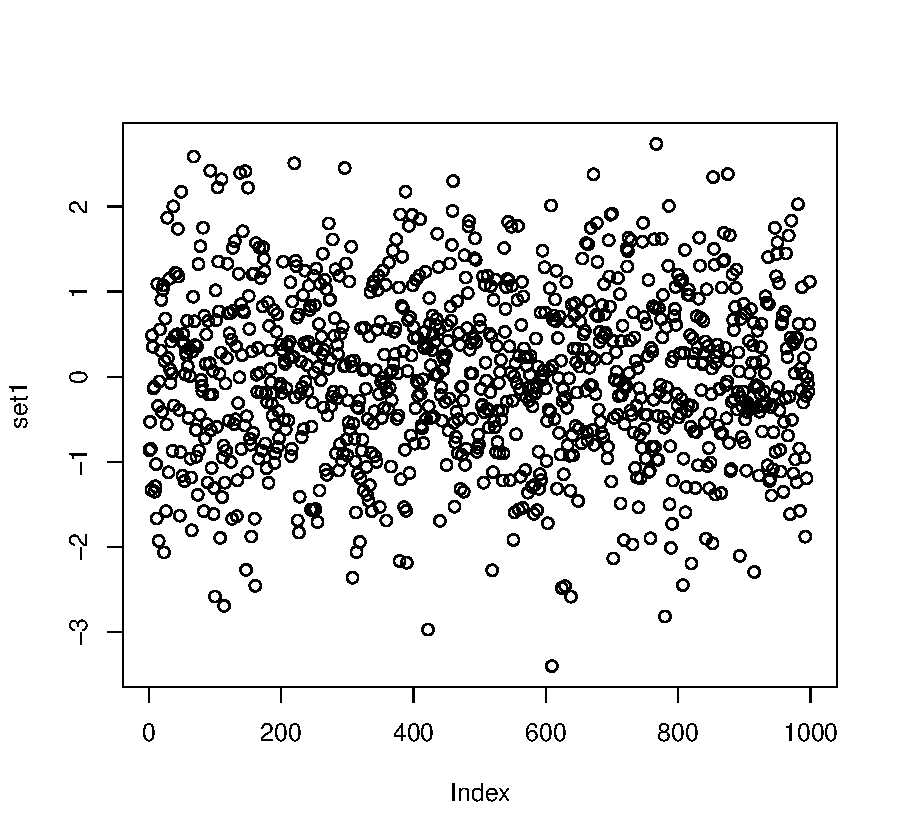
\includegraphics{plots/hist-003}
  \end{centering} 
  \end{figure}
\end{frame}

\begin{frame}[allowframebreaks, fragile]
  \frametitle{\pl{hist}}
  \begin{itemize}
  \item La forma de hacer este \emph{aplastamiento} es con una l�nea representando la densidad o con un histograma
  usando la funci�n \BIOCfunction{hist}. Si tienen curiosidad, hay funciones alternativas cuando su set de datos es
  peque�o.
  \begin{enumerate}
    \item \BIOCfunction{stripchart}
    \item \BIOCfunction{dotchart}
  \end{enumerate}
  \item Tengan cuidado, ya que un histograma es sensible al tama�o de cada barra que uses. En \pl{R} el tama�o lo escoge
  autom�ticamente, aunque pueden utilizar el argumento \alert{breaks} para hacerlo de forma manual.
  \item 
\begin{Schunk}
\begin{Sinput}
> `?`(hist)
> hist(set1)
\end{Sinput}
\end{Schunk}
  \end{itemize}
\end{frame}

\begin{frame}[fragile]
  \frametitle{Ejemplo con set1}
  \begin{figure}[htbp] 
  \begin{centering}   
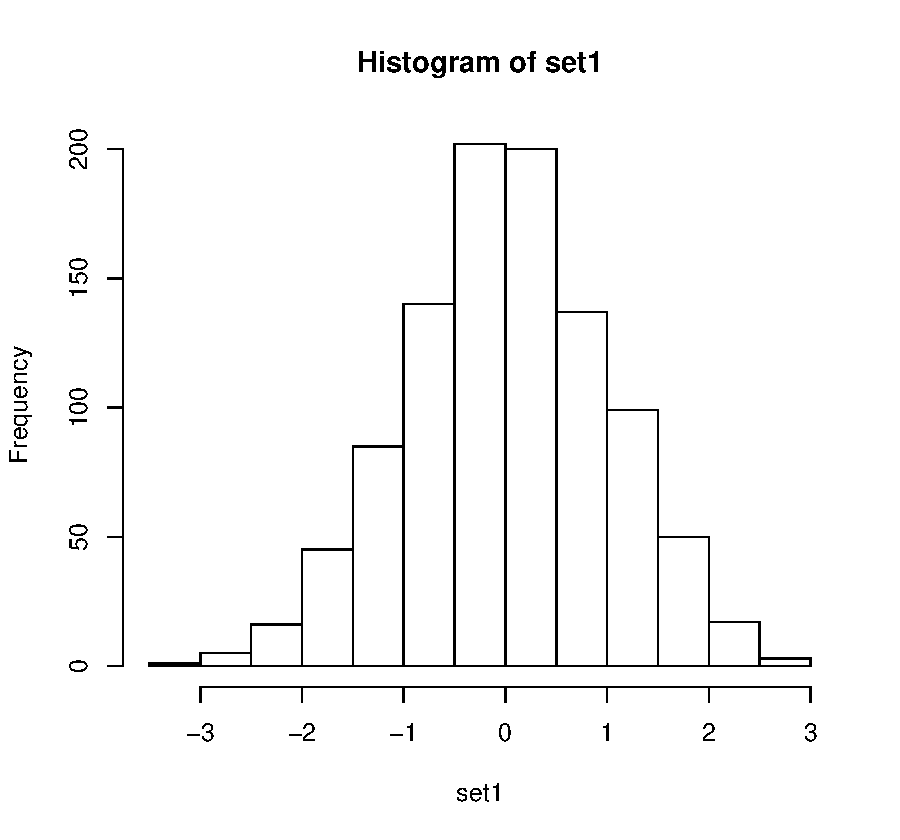
\includegraphics{plots/hist-005}
  \end{centering} 
  \end{figure}
\end{frame}

\begin{frame}[allowframebreaks, fragile]
  \frametitle{Frecuencia o prob}
  \begin{itemize}
  \item En el modo \emph{default} obtenemos un histograma de frecuencias. Podemos obtener un histograma de probabilidades usando el argumento \pl{prob=TRUE}
  \item Al igual que con otras funciones de gr�ficas pueden cambiar el color, t�tulo, etc.
  \item El siguiente ejemplo es con datos de \pl{R} y es una distribuci�n bimodal. 
\begin{Schunk}
\begin{Sinput}
> hist(faithful$waiting, col = "light blue", 
+     main = "Histograma de faithful$waiting", 
+     xlab = "Tiempo de espera entre erupciones", 
+     ylab = "Probabilidad", prob = T)
\end{Sinput}
\end{Schunk}
  \end{itemize}
\end{frame}

\begin{frame}[fragile]
  \frametitle{Otro ejemplo}
  \begin{figure}[htbp] 
  \begin{centering}   
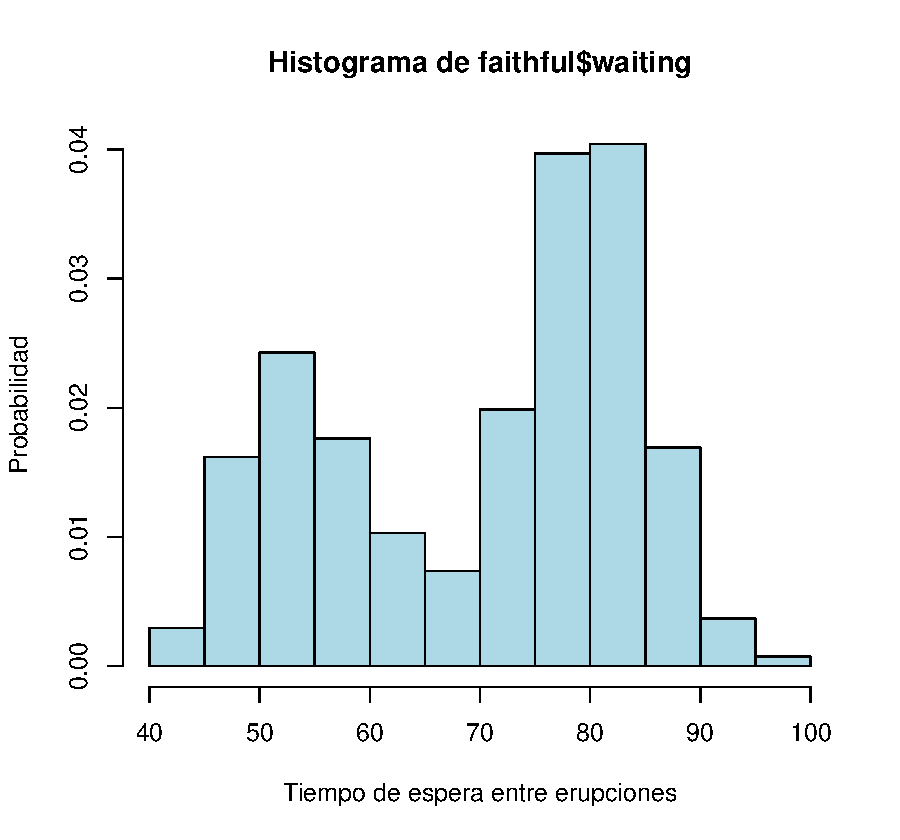
\includegraphics{plots/hist-007}
  \end{centering} 
  \end{figure}
\end{frame}


%%%%%%%%%%%%%%%%%%%%%%%%%%%%%%%%%%%%%%%%%%%%%%%%%%%%%%%%%%%%%%%%%%%%%%%%%%%
\section{Comparar distribuciones}

\begin{frame}[allowframebreaks, fragile]
  \frametitle{Usando par y mfrow}
  \begin{itemize}
  \item Usando histogramas, una forma sencilla de comparar distribuciones es hacer 2 gr�ficas pegadas usando \BIOCfunction{par}. Claro, tengan cuidado porque diferentes distribuciones
  se pueden parecer mucho bajo ciertos par�metros.
\begin{Schunk}
\begin{Sinput}
> par(mfrow = c(1, 2))
> hist(set1, prob = T)
> hist(set2, prob = T)
> par(mfrow = c(1, 1))
\end{Sinput}
\end{Schunk}
  \end{itemize}
\end{frame}

\begin{frame}[fragile]
  \frametitle{Set1 vs Set2}
  \begin{figure}[htbp] 
  \begin{centering}   
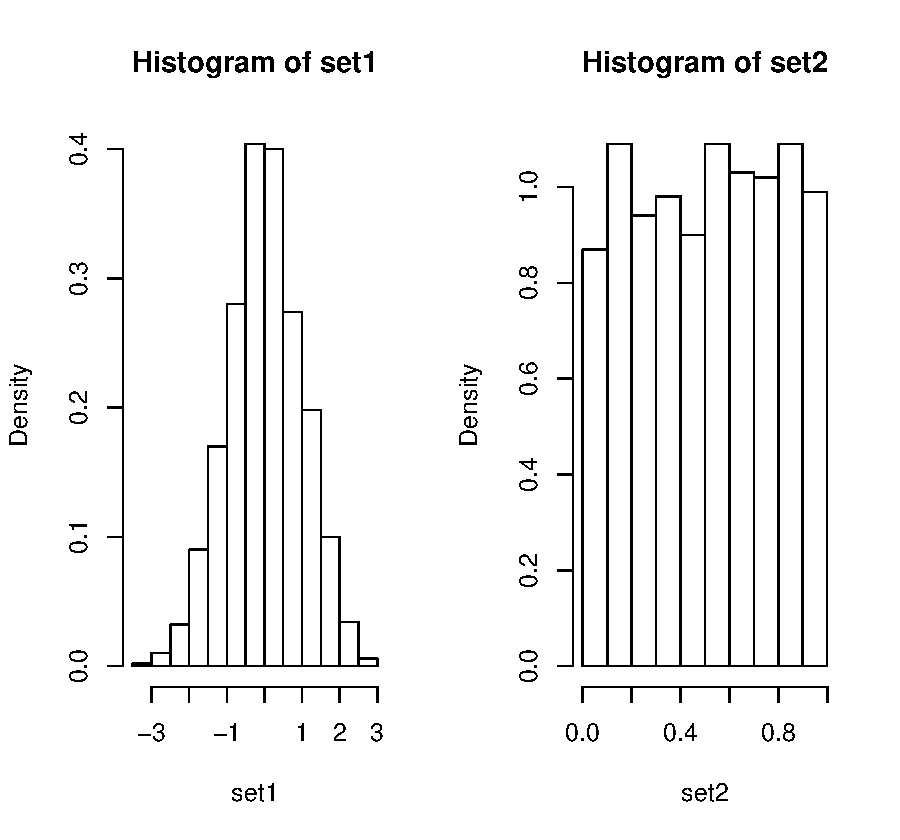
\includegraphics{plots/hist-009}
  \end{centering} 
  \end{figure}
\end{frame}

\begin{frame}[allowframebreaks, fragile]
  \frametitle{Density con Hist}
  \begin{itemize}
  \item Lamentablemente no se pueden poner 2 histogramas en una sola gr�fica, aunque en teor�a podemos utilizar las funciones \BIOCfunction{lines} junto con
  \BIOCfunction{density} para esquivar este problema.
  \item Primero les muestro una donde la l�nea es de la misma distribuci�n y luego otra donde no
\begin{Schunk}
\begin{Sinput}
> hist(faithful$waiting, prob = TRUE, 
+     ylab = "Prob", col = "light blue")
> lines(density(faithful$waiting), 
+     col = "red")
> set3 <- runif(100, 40, 70)
> hist(faithful$waiting, prob = TRUE, 
+     ylab = "Prob", col = "light blue")
> lines(density(set3), col = "red")
\end{Sinput}
\end{Schunk}
  \end{itemize}
\end{frame}

\begin{frame}[fragile]
  \frametitle{Iguales}
  \begin{figure}[htbp] 
  \begin{centering}   
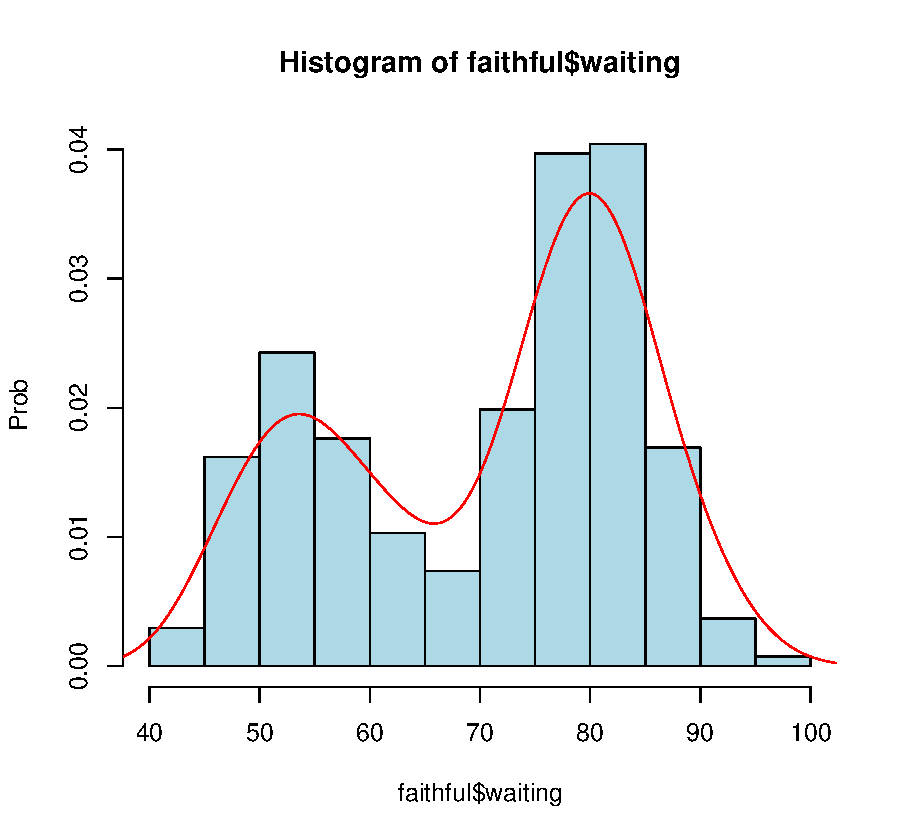
\includegraphics{plots/hist-011}
  \end{centering} 
  \end{figure}
\end{frame}

\begin{frame}[fragile]
  \frametitle{faithful vs set3}
  \begin{figure}[htbp] 
  \begin{centering}   
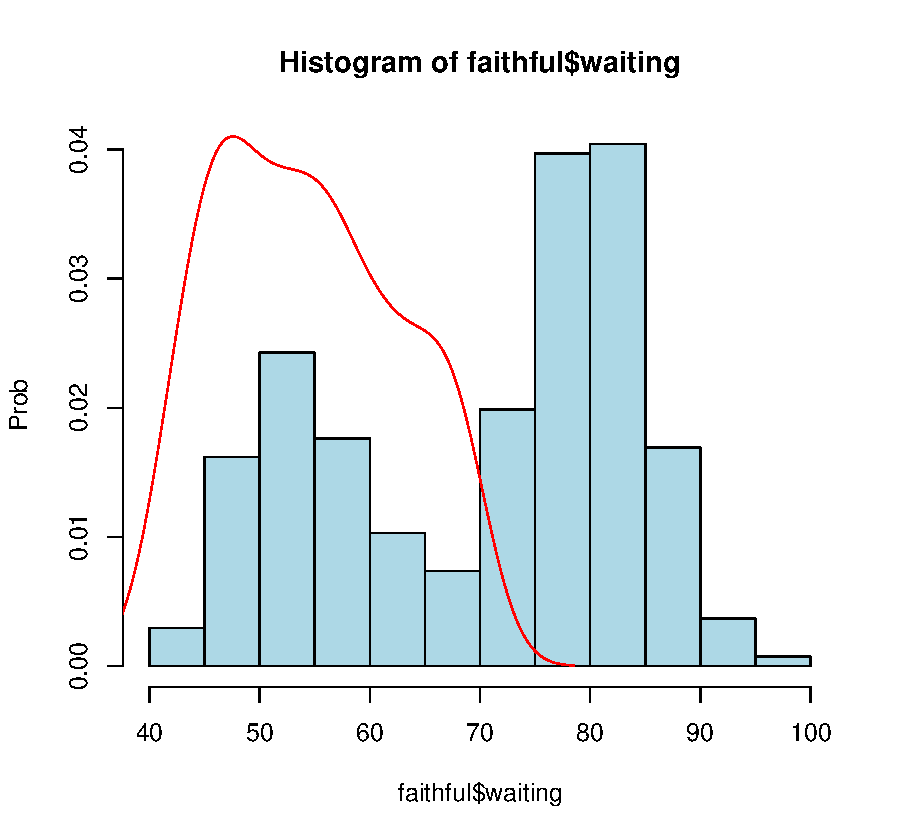
\includegraphics{plots/hist-012}
  \end{centering} 
  \end{figure}
\end{frame}

\begin{frame}[allowframebreaks, fragile]
  \frametitle{Con 2 l�neas}
  \begin{itemize}
  \item Como se han de imaginar, otra forma es usar un espacio en blanco con dos l�neas.
\begin{Schunk}
\begin{Sinput}
> plot(0, 0, ylim = c(0, 1), xlim = c(min(set1), 
+     max(set1)))
> lines(density(set1), col = "red")
> lines(density(set2), col = "blue")
\end{Sinput}
\end{Schunk}
  \end{itemize}
\end{frame}


 \begin{frame}[fragile]
  \frametitle{Set1 vs Set2}
  \begin{figure}[htbp] 
  \begin{centering}   
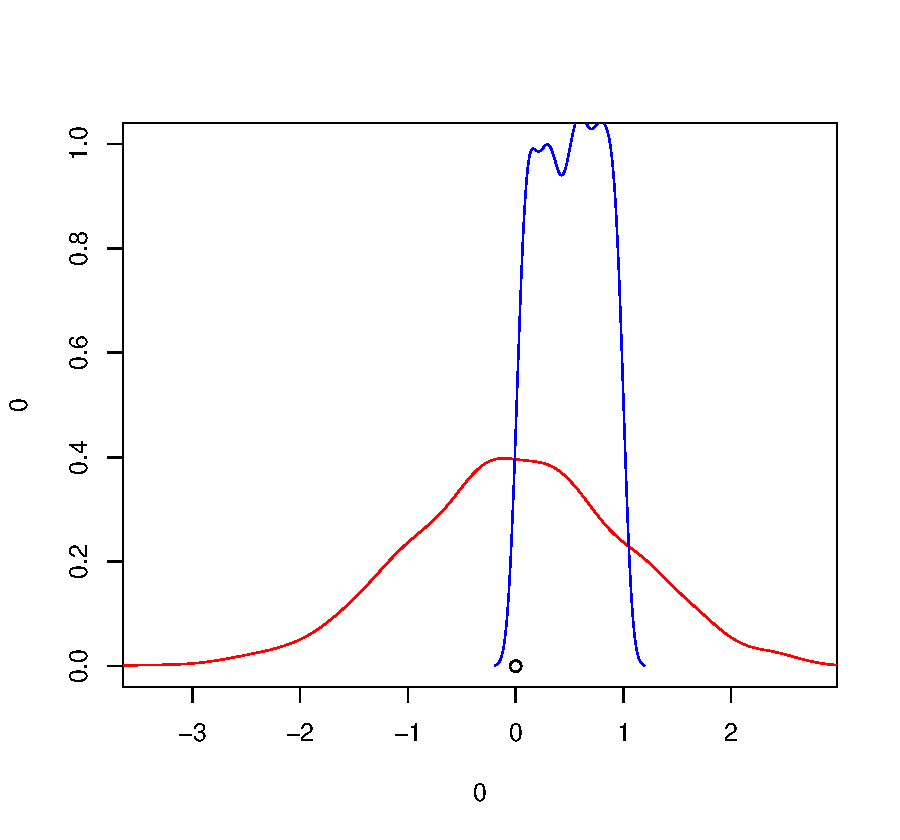
\includegraphics{plots/hist-014}
  \end{centering} 
  \end{figure}
\end{frame}

%%%%%%%%%%%%%%%%%%%%%%%%%%%%%%%%%%%%%%%%%%%%%%%%%%%%%%%%%%%%%%%%%%%%%%%%%%%
\section{Comparar cuantiles}

\begin{frame}[allowframebreaks, fragile]
  \frametitle{Q-Q plot}
  \begin{itemize}
  \item La forma \emph{pro} usando gr�ficas para comparar dos distribuciones es con la llamada "Q-Q plot". Este tipo de gr�ficas usa como informaci�n los cuantiles de las dos
  distribuciones que vas a comparar.Puede que estes comparando una muestra contra una distribuci�n te�rica, dos muestras o dos distribuciones te�ricas. Adem�s,
  tiene la ventaja de que el tama�o de tus 2 poblaciones no importa.
  \item En \pl{R} la funci�n que hace este tipo de gr�ficas es \BIOCfunction{qqplot}.
  \item Veamos como se ve set1 vs set1 y set1 vs set2.
\begin{Schunk}
\begin{Sinput}
> qqplot(set1, set1)
> qqplot(set1, set2)
\end{Sinput}
\end{Schunk}
  \end{itemize}
\end{frame}

\begin{frame}[fragile]
  \frametitle{Set1 vs Set1}
  \begin{figure}[htbp] 
  \begin{centering}   
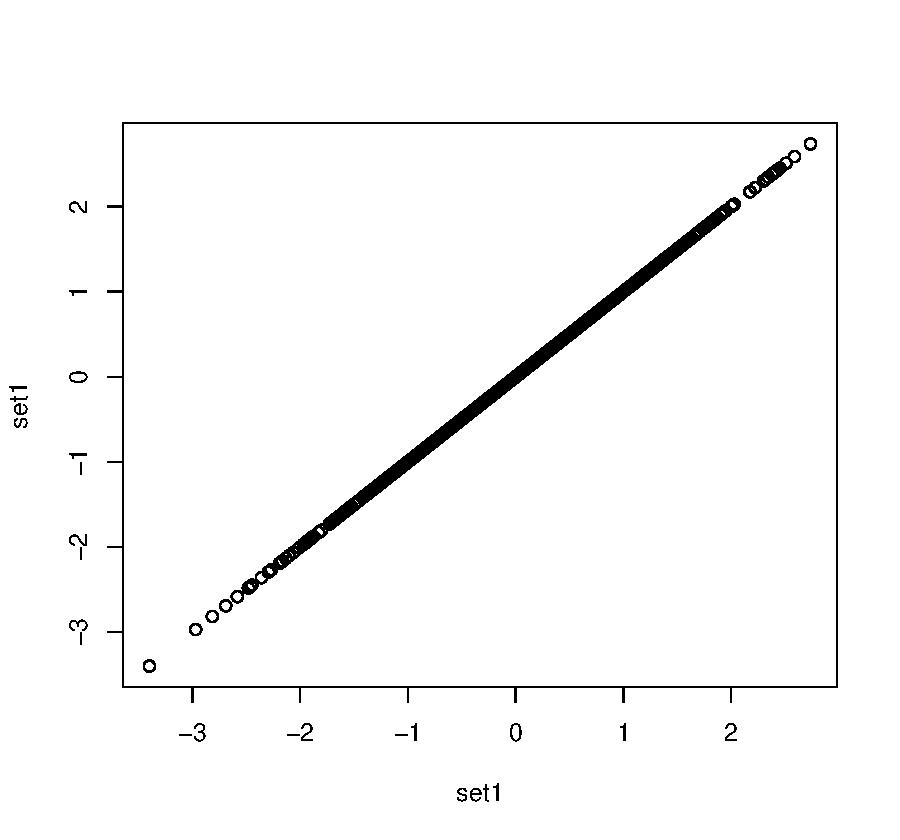
\includegraphics{plots/hist-016}
  \end{centering} 
  \end{figure}
\end{frame}

\begin{frame}[fragile]
  \frametitle{Set1 vs Set2}
  \begin{figure}[htbp] 
  \begin{centering}   
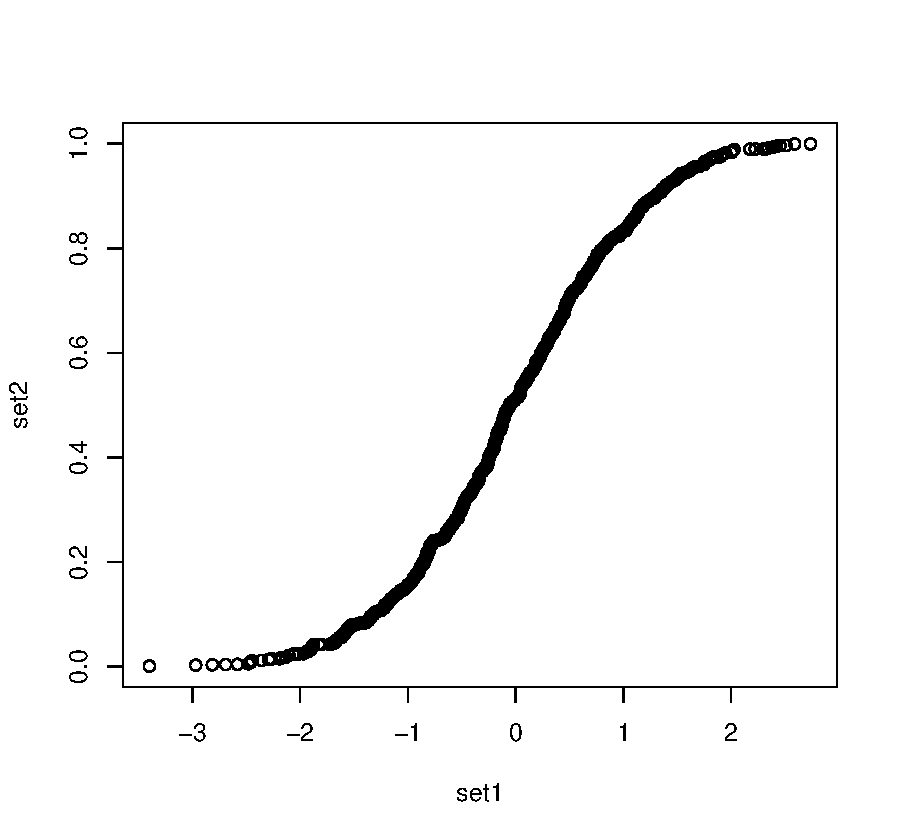
\includegraphics{plots/hist-017}
  \end{centering} 
  \end{figure}
\end{frame}

\begin{frame}[allowframebreaks, fragile]
  \frametitle{Q-Q Norm}
  \begin{itemize}
  \item Como ya vieron, si obtenemos una diagonal esta nos indica que las dos distribuciones son parecidas o iguales si nos da una diagonal
  perfecta.
  \item Ahora, digamos que tienen un set de datos y quieren saber si se distribuyen como normal.
  \item Para este caso existe la funci�n \BIOCfunction{qqnorm} la cual compara los cuantiles de tu muestra contra los cuantiles de la normal te�rica.
  \item Chequemos los siguientes ejemplos:
\begin{Schunk}
\begin{Sinput}
> set4 <- rchisq(100, 3)
> qqnorm(set4)
> qqnorm(set1)
\end{Sinput}
\end{Schunk}
  \end{itemize}
\end{frame}

\begin{frame}[fragile]
  \frametitle{QQnorm set4}
  \begin{figure}[htbp] 
  \begin{centering}   
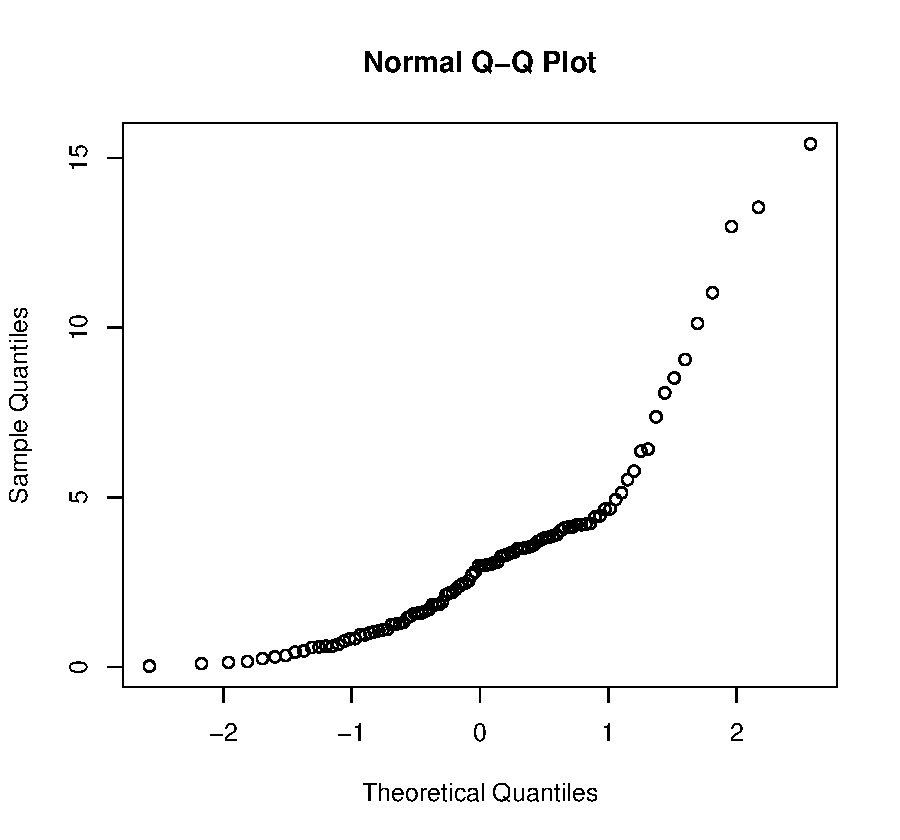
\includegraphics{plots/hist-019}
  \end{centering} 
  \end{figure}
\end{frame}

\begin{frame}[fragile]
  \frametitle{QQnorm set1}
  \begin{figure}[htbp] 
  \begin{centering}   
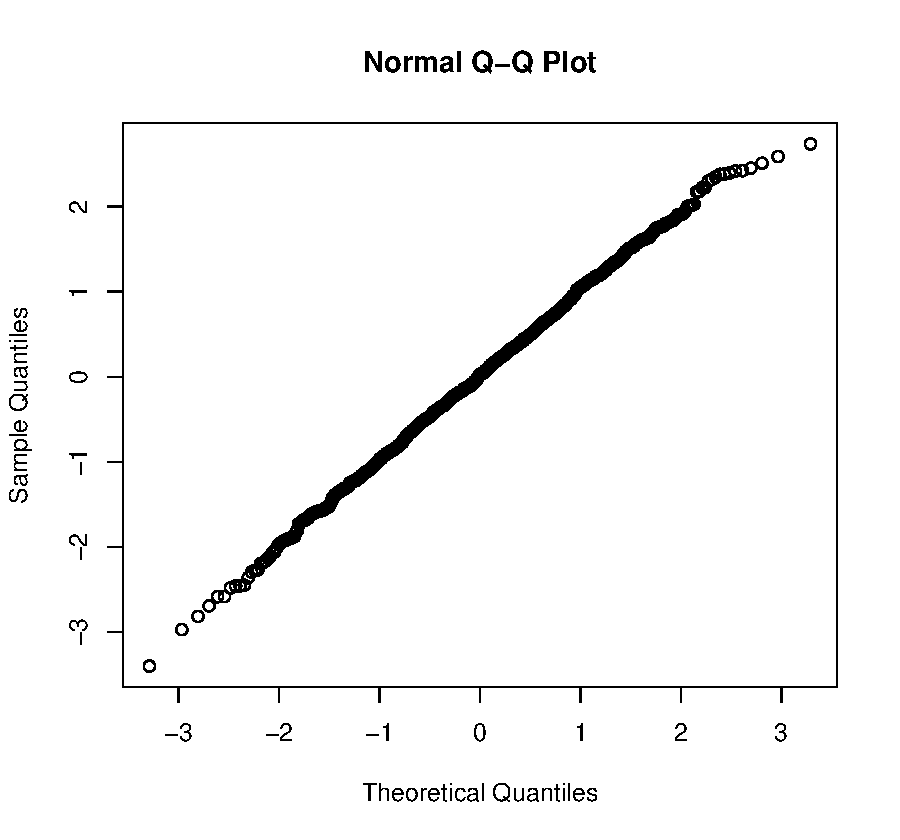
\includegraphics{plots/hist-020}
  \end{centering} 
  \end{figure}
\end{frame}

\begin{frame}[allowframebreaks]
  \frametitle{Terminando}
  \begin{itemize}
  \item Recuerden que nuestro set1 son datos que obtuvimos con \alert{rnorm} mas no obtenemos una diagonal perfecta con \pl{qqnorm}.
  \item Si se fijan, en el centro si existe nuestra diagonal pero en los bordes se curvea. Esto es por que tenemos valores extremos y es muy dif�cil que estos
  correspondan a los valores extremos te�ricos :P
  \end{itemize}
\end{frame}

\begin{frame}[allowframebreaks]
  \frametitle{Tarea}
  \begin{itemize}
  \item Asistir al evento de ma�ana jueves :)
  \item Hacer un reporte estad�stico donde comparen la cantidad de "l�quido" ingerido por la poblaci�n de la LCG en este evento vs un evento promedio.
  \item Suerte!!!
  \end{itemize}
\end{frame}

%%%%%%%%%%%%%%%%%%%%%%%%%%%%%%%%%%%%%%%%%%%%%%%%%%%%%%%%%%%%%%%%%%%%%%%%%%%

\end{document}

